%% For double-blind review submission, w/o CCS and ACM Reference (max submission space)
\documentclass[sigplan,10pt,review,anonymous]{acmart}\settopmatter{printfolios=true,printccs=false,printacmref=false}
%% For double-blind review submission, w/ CCS and ACM Reference
%\documentclass[sigplan,10pt,review,anonymous]{acmart}\settopmatter{printfolios=true}
%% For single-blind review submission, w/o CCS and ACM Reference (max submission space)
%\documentclass[sigplan,10pt,review]{acmart}\settopmatter{printfolios=true,printccs=false,printacmref=false}
%% For single-blind review submission, w/ CCS and ACM Reference
%\documentclass[sigplan,10pt,review]{acmart}\settopmatter{printfolios=true}
%% For final camera-ready submission, w/ required CCS and ACM Reference
%\documentclass[sigplan,10pt]{acmart}\settopmatter{}

\usepackage[utf8]{inputenc}
\usepackage[english]{babel}
\RequirePackage[outputdir=latex.out,cache=false]{minted}
\usepackage{microtype}
\usepackage{hyperref}
\usepackage{xspace}
\usepackage{graphicx}
\usepackage{url}
\usepackage{amsmath}
\usepackage{amssymb}
\usepackage{amsthm}

%% \setmonofont[Scale=MatchLowercase]{DejaVu Sans Mono}
%% \setmonofont{DejaVu Sans Mono}

\microtypecontext{spacing=nonfrench}
\microtypesetup{
  final,
  tracking=true,
  kerning=true,
  spacing=true,
  factor=1100,
  stretch=20,
  shrink=20
}
\SetTracking{encoding={*}, shape=sc}{0} % No tracking for smallcaps


\newcommand{\Mesh}{\textsc{Mesh}\xspace}


%% Conference information
%% Supplied to authors by publisher for camera-ready submission;
%% use defaults for review submission.
\acmConference[PLDI'18]{ACM SIGPLAN Conference on Programming Language Design and Implementation}{June 18--22, 2018}{Philadelphia, PA, USA}
\acmYear{2018}
\acmISBN{} % \acmISBN{978-x-xxxx-xxxx-x/YY/MM}
\acmDOI{} % \acmDOI{10.1145/nnnnnnn.nnnnnnn}
\startPage{1}

%% Copyright information
%% Supplied to authors (based on authors' rights management selection;
%% see authors.acm.org) by publisher for camera-ready submission;
%% use 'none' for review submission.
\setcopyright{none}
%\setcopyright{acmcopyright}
%\setcopyright{acmlicensed}
%\setcopyright{rightsretained}
%\copyrightyear{2017}           %% If different from \acmYear

%% Bibliography style
\bibliographystyle{ACM-Reference-Format}
%% Citation style
%\citestyle{acmauthoryear}  %% For author/year citations
%\citestyle{acmnumeric}     %% For numeric citations
%\setcitestyle{nosort}      %% With 'acmnumeric', to disable automatic
                            %% sorting of references within a single citation;
                            %% e.g., \cite{Smith99,Carpenter05,Baker12}
                            %% rendered as [14,5,2] rather than [2,5,14].
%\setcitesyle{nocompress}   %% With 'acmnumeric', to disable automatic
                            %% compression of sequential references within a
                            %% single citation;
                            %% e.g., \cite{Baker12,Baker14,Baker16}
                            %% rendered as [2,3,4] rather than [2-4].


%%%%%%%%%%%%%%%%%%%%%%%%%%%%%%%%%%%%%%%%%%%%%%%%%%%%%%%%%%%%%%%%%%%%%%
%% Note: Authors migrating a paper from traditional SIGPLAN
%% proceedings format to PACMPL format must update the
%% '\documentclass' and topmatter commands above; see
%% 'acmart-pacmpl-template.tex'.
%%%%%%%%%%%%%%%%%%%%%%%%%%%%%%%%%%%%%%%%%%%%%%%%%%%%%%%%%%%%%%%%%%%%%%


%% Some recommended packages.
\usepackage{booktabs}   %% For formal tables:
                        %% http://ctan.org/pkg/booktabs
\usepackage{subcaption} %% For complex figures with subfigures/subcaptions
                        %% http://ctan.org/pkg/subcaption


\begin{document}

%% Title information
\title[Mesh]{Immovable Objects Meet An Irresistible Force: Meshing Memory Management for Compaction without Relocation}         %% [Short Title] is optional;
                                        %% when present, will be used in
                                        %% header instead of Full Title.
%\titlenote{with title note}             %% \titlenote is optional;
                                        %% can be repeated if necessary;
                                        %% contents suppressed with 'anonymous'
%\subtitle{Subtitle}                     %% \subtitle is optional
%\subtitlenote{with subtitle note}       %% \subtitlenote is optional;
                                        %% can be repeated if necessary;
                                        %% contents suppressed with 'anonymous'


%% Author information
%% Contents and number of authors suppressed with 'anonymous'.
%% Each author should be introduced by \author, followed by
%% \authornote (optional), \orcid (optional), \affiliation, and
%% \email.
%% An author may have multiple affiliations and/or emails; repeat the
%% appropriate command.
%% Many elements are not rendered, but should be provided for metadata
%% extraction tools.

%% Author with single affiliation.
\author{First1 Last1}
\authornote{with author1 note}          %% \authornote is optional;
                                        %% can be repeated if necessary
\orcid{nnnn-nnnn-nnnn-nnnn}             %% \orcid is optional
\affiliation{
  \position{Position1}
  \department{Department1}              %% \department is recommended
  \institution{Institution1}            %% \institution is required
  \streetaddress{Street1 Address1}
  \city{City1}
  \state{State1}
  \postcode{Post-Code1}
  \country{Country1}                    %% \country is recommended
}
\email{first1.last1@inst1.edu}          %% \email is recommended

%% Author with two affiliations and emails.
\author{First2 Last2}
\authornote{with author2 note}          %% \authornote is optional;
                                        %% can be repeated if necessary
\orcid{nnnn-nnnn-nnnn-nnnn}             %% \orcid is optional
\affiliation{
  \position{Position2a}
  \department{Department2a}             %% \department is recommended
  \institution{Institution2a}           %% \institution is required
  \streetaddress{Street2a Address2a}
  \city{City2a}
  \state{State2a}
  \postcode{Post-Code2a}
  \country{Country2a}                   %% \country is recommended
}
\email{first2.last2@inst2a.com}         %% \email is recommended
\affiliation{
  \position{Position2b}
  \department{Department2b}             %% \department is recommended
  \institution{Institution2b}           %% \institution is required
  \streetaddress{Street3b Address2b}
  \city{City2b}
  \state{State2b}
  \postcode{Post-Code2b}
  \country{Country2b}                   %% \country is recommended
}
\email{first2.last2@inst2b.org}         %% \email is recommended


%% Abstract
%% Note: \begin{abstract}...\end{abstract} environment must come
%% before \maketitle command
\begin{abstract}
\begin{abstract}
Because C and C++ objects cannot be relocated, memory allocators for
those languages cannot compact objects and thus can suffer potentially
catastrophic fragmentation. In a classic result, Robson showed that
such allocators can consume up to $(O \log M/m)$, where $M/m$ is the
ratio of the largest and smallest object request
sizes~\cite{robson1977worst}. We present a counterintuitive result: a
memory management algorithm that can perform compaction without
relocating objects. Our approach \emph{meshes} together objects from
separate pages whose virtual offsets do not overlap, compacting them
physically onto a single page while maintaining their virtual
addresses. Meshing depends on widely-available OS support and a
randomized algorithm that provides provably effective compaction with
high probability. We demonstrate that meshing is practical and
effective by implementing a prototype meshing memory allocator.
\end{abstract}

\end{abstract}


%% 2012 ACM Computing Classification System (CSS) concepts
%% Generate at 'http://dl.acm.org/ccs/ccs.cfm'.
\begin{CCSXML}
<ccs2012>
<concept>
<concept_id>10011007.10011006.10011008</concept_id>
<concept_desc>Software and its engineering~General programming languages</concept_desc>
<concept_significance>500</concept_significance>
</concept>
<concept>
<concept_id>10003456.10003457.10003521.10003525</concept_id>
<concept_desc>Social and professional topics~History of programming languages</concept_desc>
<concept_significance>300</concept_significance>
</concept>
</ccs2012>
\end{CCSXML}

\ccsdesc[500]{Software and its engineering~General programming languages}
\ccsdesc[300]{Social and professional topics~History of programming languages}
%% End of generated code


\keywords{Mesh, meshing, compaction, memory management, unmanaged languages}


\maketitle


\section{Introduction}
\label{sec:introduction}

In unmanaged languages like C and C++ the memory addresses of objects
are directly exposed to the program, and as a result objects cannot be
relocated.  These languages let programmers store addresses in
integers, perform arithmetic on addresses, write them to and from
pipes, and convert integers into addresses.  Given such an adversarial
environment, a runtime system can not guarantee that it can identify
all object references at any given point in time.  Without precisely
identifying \textit{all} references objects can not safely be
relocated, as all locations that point to a moved object need to be
updated for the program to continue executing correctly.

Because objects can not be relocated, memory allocators for these
languages can not perform compaction and thus programs may suffer from
fragmentation.  Fragmentation is a result of the fact that while a
user's program manages memory at the granularity of \textit{bytes},
operating systems manage memory at the level of \textit{pages} (4 KiB
on most contemporary architectures).  Fragmentation occurs when a
small number of program objects require the reservation of a
corresponding large number of pages from the operating system.
Fragmentation can result in a program requiring orders of magnitude
more memory from the operating system than is required by the
semantics of the program.

Fragmentation is important because it exacerbates memory pressure --
one of the scarcest resources on modern computing devices.  70 percent
of Google Chrome crashes on low-RAM Android devices are caused by
Chrome running out of memory when attempting to display the
page~\cite{hara:whymemory}.  Embedded systems designed for the
Internet-of-Things (IoT), such as the Raspberry Pi Zero W, ship with
wireless networking, 3D graphics, and complete operating system stacks
but only hundreds of megabytes of memory~\cite{rpi:zero}.

Fragmentation has been widely
studied~\cite{johnstone:1998:fragmentation} and solved for managed
languages with \textit{moving
  compaction}~\cite{hansen:1969:compaction,fenichel:1969:compaction}
in the late 1960s.  Compaction minimizes fragmentation by moving live
objects close together.  Contemporary runtimes like the Hotspot
JVM~\cite{microystems2006memory}, The .NET
VM~\cite{microsoft:dotnet-gc}, the SpiderMonkey JavaScript
VM~\cite{mozilla:spidermonkey-compaction} and others implement moving
compaction as part of their garbage collection algorithms.

We present \Mesh, the first runtime system to bring precise compaction
to unmanaged languages like C and C++.  \Mesh uses randomization to
provably bound the impact of fragmentation with high probability.

\subsection{Contributions}
\label{sec:contributions}

This paper makes the following contributions:

\begin{itemize}
\item It introduces the concept of \textbf{meshing}, a mechanism that
  provides \textit{compaction without relocation} for unmanaged
  languages.  Meshing eliminates memory fragmentation in languages
  like C and C++ with high probability, and we identify analytic
  bounds on the savings possible and achievable.
\item It presents \textbf{\Mesh}, a runtime system and memory
  allocator that delivers compaction without relocation for binaries
  compiled from unmanaged languages like C, C++ and Rust.  We evaluate
  \Mesh's performance empirically and analytically.
  % TODO: mention evaluation results
\end{itemize}

The rest of this paper is organized as follows.
Section~\ref{sec:meshing} introduces the concept of meshing and show
how our approach reduces fragmentation in a representative unmanaged
program.  Section~\ref{sec:allocator} details \Mesh's efficient memory
allocator.  Section~\ref{sec:theory} presents the theoretical results
that make meshing efficient and
practical. Section~\ref{sec:evaluation} provides an empirical
evaluation of \Mesh, and section~\ref{sec:discussion} discusses how
several classes of applications would benefit from deeper integration
with \Mesh.  Finally, section~\ref{sec:related-work} discusses related
work, and section~\ref{sec:conclusion} concludes this paper.


\section{Overview}
\label{sec:meshing}

\begin{figure}[!t]
\centering
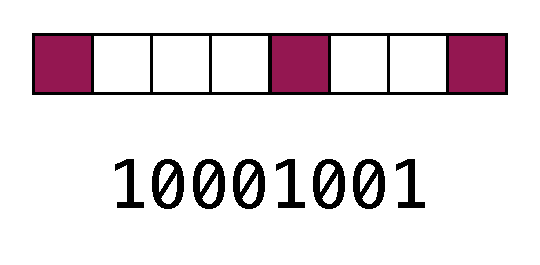
\includegraphics[width=.3\textwidth]{figures/bitmap_bitstring}
\caption{The bitmaps managing the allocated space in a span
  (visualized as allocated objects in the span, top) can be
  represented as bitstrings of 0s and 1s (bottom), where a 1
  corresponds to an allocated object and 0 to free space.}
\label{fig:bitmap-bitstring}
\end{figure}

Meshing is the problem and process of minimizing physical memory use
(measured as resident-set size, or RSS) without modifying allocated
virtual addresses.

A \textit{span} is a contiguous region of memory, and the size of a
span is a multiple of the page size between 4 KiB and 128 KiB.  Each
span allocates objects of a single-size only, for example a 4 KiB span
might hold 32 objects of size 128 bytes.  We can represent a span by a
\textit{bitstring}, a string with a 1 for an allocated object at that
offset from the start of the span and 0 otherwise.  The length of the
bitstring is the number of objects that span holds.

We say $t$ spans \textit{mesh} iff the logical-AND of their bitstrings
($s_i$) of length $t$ is zero. INCORRECT? THIS LETS US MESH TWO 11111 STRINGS WITH ONE 00000 STRING FOR INSTANCE. Formally:

\begin{align}
  \forall k \in [0, b-1]. \sum_{0 \leq i \leq t} s_i[k] \leq 1
\end{align}

This definition characterizes the constraints of the technique by which 
meshing is possible, wherein two or more spans are meshed or "stacked" 
on top of each other.  Each object in the resulting meshed span resides at the same 
offset as it did in its original span, as in Figure 2.  This is only possible when no two spans
have objects at the same offset.  After this process all objects reside
in a single span, and all other spans are empty and can be used anew
for allocation.

The layout and management of a program's heap guide how we consider
meshing.  In a running program, the heap is managed as a number of
different \textit{size classes} along with a region consisting of
large allocations.  Allocations are fulfilled from the smallest size
class they fit in (e.g. an allocation request for 50 bytes is
satisfied by the 64-byte size class), and objects larger than 16 KiB
are individually served from the large allocation region.

We treat each size class as an independent instance of the meshing
problem, and large allocations are not meshed.  As large allocations
are all many multiples of the page size significant fragmentation
between them does not exist.  The number of size-classes is fixed at
compilation time and constant during the execution of a program.

From here, we consider meshing as dealing with a single size-class,
and refer to all spans within this size class as $S$.  If we want to
mesh the entire heap, this means solving $n$ instances of the meshing
problem, where $n$ is the number of size classes.


\begin{figure}[!t]
  \centering
  \begin{subfigure}[t]{.5\textwidth}
    \centering
    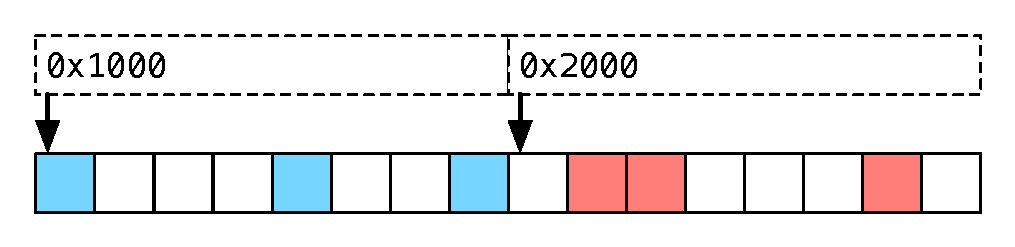
\includegraphics[width=\textwidth]{figures/before_meshing}
    \caption{Two adjacent spans that are candidates for meshing.}
  \end{subfigure}%
  ~

  \begin{subfigure}[t]{.5\textwidth}
    \centering
    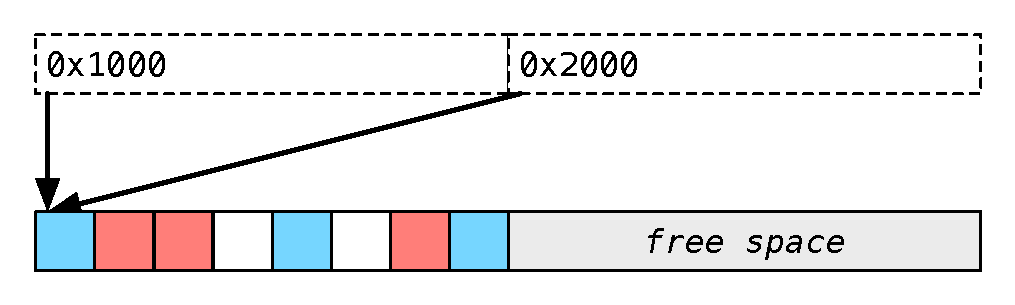
\includegraphics[width=\textwidth]{figures/after_meshing}
    \caption{After meshing, both virtual spans refer to the same
      physical \newline span, with live objects interleaved.}
  \end{subfigure}
  \caption{Virtual and physical memory layout before and after
    meshing.  After meshing, physical span occupancy has increased
    from 37.5\% to 75\% and one physical span has been returned to the
    OS for reuse.}
  \label{fig:meshing}
\end{figure}

Finally, meshing relies on the fact that there are two types of spans,
virtual and physical.  A \textit{virtual} span refers to the memory
addresses visible to the program being executed, while a
\textit{physical} span corresponds to the area in memory where
allocated objects live.  Meshing is concerned with minimizing the
count of in-use physical spans without modifying or moving virtual
spans.  As noted in Section~\ref{sec:introduction}, we cannot change
or modify virtual addresses returned from the allocator, as we do
not have a way to enumerate and update all references the program has
stored.  Since the last two digits of a virtual address directly specify the offset of the referenced object in the span, objects cannot
be safely relocated to a different offset, leading to our 

Allocated objects and free space within a span are tracked by the
memory allocator as a bitmap (see Section~\ref{sec:allocator}) -- the
in-memory representation of a bitstring.  For example, for objects of
size 32 and a span size of 4 KiB, the span can hold 128 32-byte
objects, so allocated objects are be tracked with a 128-bit bitmap.
Each allocated object in a running program has a unique
\textit{(bitmap, offset)} tuple.  Bitmaps are between 8 and 256-bits
in length.

We can therefore think of the meshing problem as that of partitioning
a set of equal-length bitstrings such that the bitstrings in each subset
mesh.  An optimal partition would minimize the number of such subsets.
This abstraction allows us to analyze the complexity of this computational
task in Section~\ref{sec:theory}.

\section{The \Mesh Allocator}
\label{sec:allocator}

\begin{figure}[!t]
  \centering
  \begin{subfigure}[t]{.5\textwidth}
    \centering
    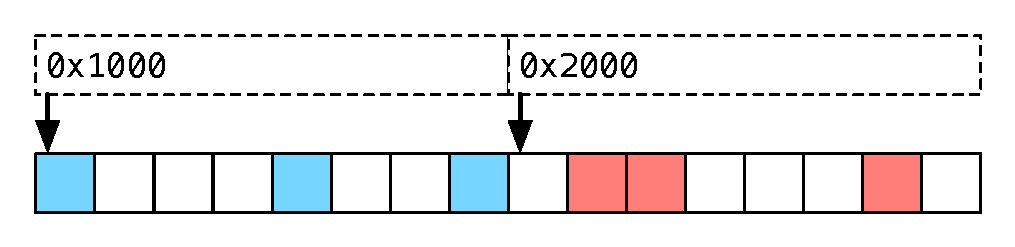
\includegraphics[width=\textwidth]{figures/before_meshing}
    \caption{Two adjacent spans that are candidates for meshing.}
  \end{subfigure}%
  ~

  \begin{subfigure}[t]{.5\textwidth}
    \centering
    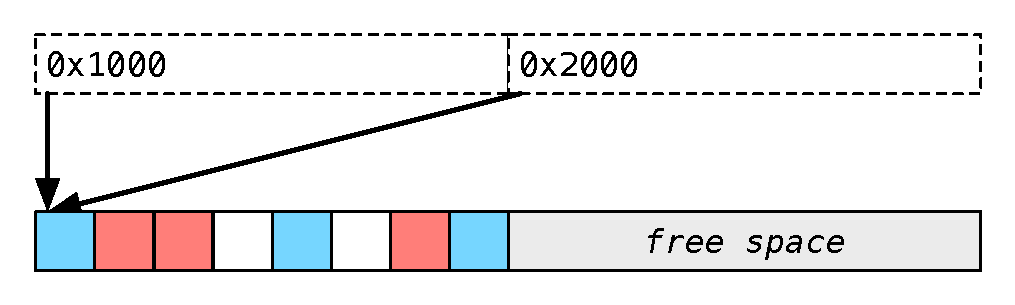
\includegraphics[width=\textwidth]{figures/after_meshing}
    \caption{After meshing, both virtual spans refer to the same
      physical \newline span, with live objects interleaved.}
  \end{subfigure}
  \caption{Virtual and physical memory layout before and after
    meshing.  After meshing, physical span occupancy has increased
    from 37.5\% to 75\% and one physical span has been returned to the
    OS for reuse.}
  \label{fig:meshing}
\end{figure}

\Mesh is a memory allocator and runtime system for Linux that provides
a drop in replacement for the standard C/C++ and POSIX allocation
functions available from libc.  Mesh can be explicitly linked against,
e.g. by passing \texttt{-lmesh} to the linker at compile time, or used
with \texttt{LD\_PRELOAD} by the dynamic linker at execution time.
When loaded, \Mesh \textit{interposes} on calls to standard libc
functions, providing alternative functionality (in the case of
\texttt{malloc}) or to do bookkeeping before invoking libc's
implementation (in the case of \texttt{pthread\_create}.

\begin{figure}
  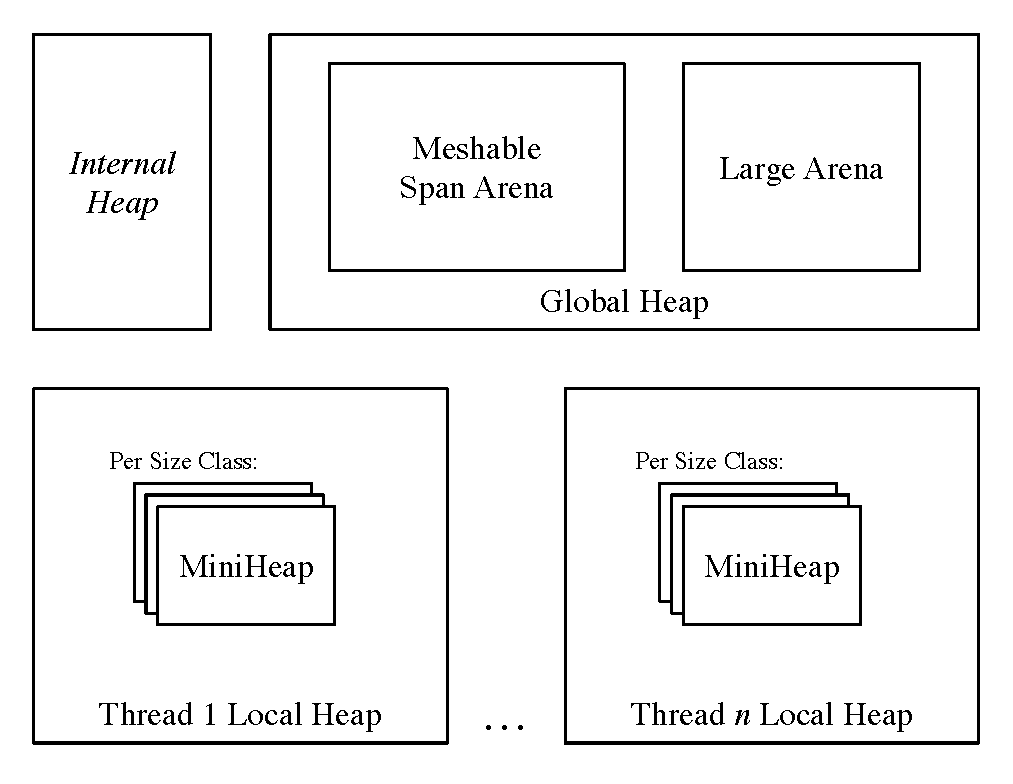
\includegraphics[width=.5\textwidth]{figures/global_heap}
  \caption{The allocator in mesh is managed by 4 main components.  The
    internal allocator provides management for \Mesh-internal dynamic
    data structures.  The global heap manages both the meshable arena
    spans are allocated out of, along with large objects.  Each thread
    has a local heap which satisfies small allocations from MiniHeaps,
    where there is one MiniHeap per size class.}
  \label{fig:global-heap}
\end{figure}

Mesh has three main components: the \textit{global heap} and runtime
state shared by all threads, \textit{thread local heaps} that can
satisfy allocations without taking locks, and MiniHeaps to track
occupancy and other metadata for spans.

Mesh is segregated-fit allocator.  Allocations are fulfilled from the
smallest size class they fit in (e.g. objects of size 32-64 bytes),
and objects larger than 16 KiB are individually served from the large
allocation region.

Spans, introduced in Section~\ref{sec:meshing}, are multiples of the
page size and contains between 8 and 256 objects of a constant size.

\subsection{MiniHeaps}

Miniheaps manage allocated physical spans of memory.  Each MiniHeap
contains metadata on the span start address and length, object size,
and allocation bitmap.  The number of objects that can be allocated
out of this bitmap is the \textit{objectCount = spanSize / objSize}.
The allocation bitmap is initialized to \textit{objectCount} zero
bits, and when an object is allocated the bit corresponding to its
offset from the start of the span is set to one.  Bitmap operations
are atomic, in order to ensure consistency without locking in
multi-threaded programs.

When a MiniHeap is allocated, there is a single virtual span that
points to the physical memory managed by the MiniHeap, and this
virtual span corresponds to the identity mapping between virtual and
physical offsets in the meshing arena.  After meshing there may be
multiple virtual spans that point to the MiniHeaps physical memory.

Miniheaps are either in-use or detached.  An in-use MiniHeap is owned
by a single local heap, while a detached MiniHeap is only referenced
by the global heap.  New objects are \textit{only} allocated out of
in-use MiniHeaps, and each in-use MiniHeap has an associated shuffle
freelists that is used to ensure fast randomized allocation.

\subsubsection{Shuffle Freelists}

\begin{figure}[!ht]
  \input{local-malloc.cc}
  \input{miniheap-malloc.cc}
  \input{local-free.cc}
  \input{miniheap-free.cc}
  \caption{Pseudocode for mesh allocation and deallocation routines.}
  \label{fig:malloc}
\end{figure}

In order to allocate objects randomly from a span in constant time, we
maintain a per-thread freelist of object offsets.  These offsets are
from the start of the span:

\vspace{-1.2em}
\begin{align*}
  \text{\textit{ptr}} = \text{\textit{spanStart + off*objSize}}
\end{align*}

This freelist is initialized with all of the available offsets $[0
  .. $ objectCount $]$ and then sorted with the Knuth-
Fischer-Yates shuffle~\cite{knuth:1981:semi}.

When an object is freed and the owning MiniHeap is still in-use, a
single iteration of the shuffle is performed to re-add the newly freed
offset back to the list of available offsets.

\begin{figure}[!t]
  \begin{subfigure}[t]{.4\textwidth}
    \centering
    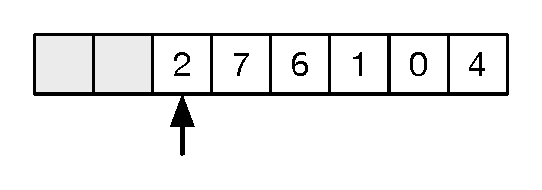
\includegraphics[width=\textwidth]{figures/shuffle-freelist_a}
    \caption{A freelist for a span of size 8, where 2 objects have
      already been allocated.}
  \end{subfigure}%
  ~

  \begin{subfigure}[t]{.4\textwidth}
    \centering
    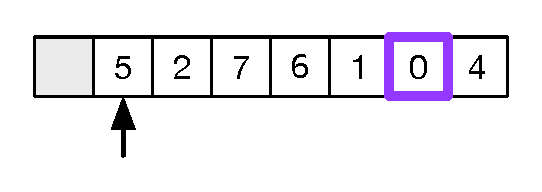
\includegraphics[width=\textwidth]{figures/shuffle-freelist_b}
    \caption{The offset is pushed on the front of the list, the list
      head pointer is updated, and a random element in [1,7] is chosen
      to swap with.}
  \end{subfigure}%
  ~

  \begin{subfigure}[t]{.4\textwidth}
    \centering
    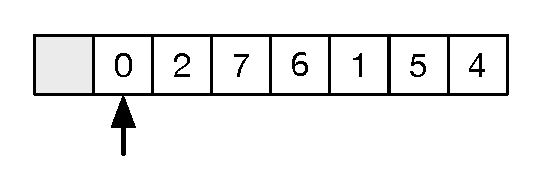
\includegraphics[width=\textwidth]{figures/shuffle-freelist_c}
    \caption{After the swap happens, new allocations proceed in a
      bump-pointer-like fashion.}
  \end{subfigure}
  \caption{Shuffle freelists enable bump-pointer-like random
    allocation out of a span.  When an object is freed and the
    MiniHeap it was allocated from is still attached to the local
    thread, its offset (5, in this example) is added back to the
    freelist with a single re-shuffle.}
  \label{fig:shuffle-freelists}
\end{figure}

Shuffle freelists are used in place of the random probing approach
used in Diehard and
Dieharder~\cite{1134000,Novark:2010:DSH:1866307.1866371}.  Random
probing works by choosing a random number in
$[0,\text{\textit{objectCount}}-1]$ and if that bit is zero in the
bitmap, setting it to one and using it as the offset for allocation.
If the offset is already one, a new random offset is chosen and the
process repeated.  Random probing allocates objects in $O(1)$ expected
time, with the catch that it requires overprovisioning memory.
Shuffle freelists solve this problem and provide $O(1)$ allocations
and frees not only in expectation, and with lower constants.

With maximum of 256 objects in a span, each offset in the freelist can
be represented as an unsigned character.  As we only need a freelist
for in-use MiniHeaps, the amount of memory required for freelists is
$256ct$, where $c$ is the number of size classes (11 in the current
implementation) and $t$ is the number of live threads, about 2.8 KiB
per thread.

\subsubsection{Locality}

Shuffle freelists give \Mesh bump-pointer like allocation speed in the
common case.  Like DieHard but unlike many other allocators, \Mesh
does not try to allocate consecutive objects nearby.  Modern 64-bit
Intel processors have 64-byte cache-lines, and ARM devices have 32 or
64-byte cache lines, meaning that object locality has little impact on
L1 cache locality.  TLB pressure should be unaffected compared to
other segregated-fit allocators with the same choice of size classes,
as for small objects we allocate randomly within a 4-KiB span, which
matches the page size.

\subsection{Thread Local Heap}

All malloc and free requests are initially handled by the thread local
heap.  The thread local heap has pointers to MiniHeaps for each size
class, a reference to the global heap, and its own random number
generator.

For small object allocations, the requested object size is converted
into a size class.  There is either an attached MiniHeap for that size
class, or a new one is requested from the global heap.  If after
allocating an object a MiniHeap is full (the freelist associated with
that MiniHeap is empty), the freelist is freed and the MiniHeap
detached from the local heap.  A new MiniHeap will be allocated the
next time an object of that size class is requested.

If the allocation request is for a large object (larger than 16 KiB),
it is forwarded on to the global heap.  Otherwise, the MiniHeap
corresponding to the size-class of the request is

A free request is either for an object in a span owned by an attached
MiniHeap, or forwarded to the global heap.

\subsection{Global Heap}

The global heap allocates new MiniHeaps for thread-local heaps,
handles all large object allocation and deallocation, performs
non-local frees for all objects, and coordinates meshing.

\subsubsection{MiniHeap allocation}

The global heap has an arena that meshable spans are allocated out of.
It is managed with a combination of a bitmap for tracking allocated
\textit{pages}, a red-black tree for retrieving the MiniHeap
corresponding to a pointer in $O(\lg{n})$ time, where $n$ is the heap
size, and per-size-class linked lists of all live MiniHeaps.

Allocating a MiniHeap involves reserving a set of $k$ consecutive
pages in the arena bitmap, allocating and initializing a new MiniHeap
instance from \Mesh's internal allocator, initializing the MiniHeap's
shuffle freelist, and recording the MiniHeap in the global red-black
tree and size-class-specific linked list.

\subsubsection{Large objects}

Large objects are allocated directly as anonymous \texttt{mmap}
mappings and returned to the OS on free with \texttt{munmap}.

As large objects are many multiples of the page size, they do not
suffer from fragmentation.

\subsubsection{Non-local frees}

If \texttt{free} is called on a pointer that does not belong to that
thread's local heap, the free is handled by the global heap.  A
read-lock is obtained, the MiniHeap is looked up in the global heap's
red-black tree of all MiniHeaps and that MiniHeap's bitmap is updated
atomically in a compare-and-set loop.

There are two reasons non-local frees may happen: enough objects of
the object's size class have occurred on the current thread that the
parent MiniHeap was exhausted and detached, or the pointer was
allocated on a remote thread.

\subsection{Meshing}

The \Mesh implementation is guided by the results in
Section~\ref{sec:meshing} to find a number of spans that can be meshed
together.

Non-local frees to the global heap initiate the meshing process with
low probability.  The reason only non-local frees may initiate a mesh
check is that frees that are able to be handled thread-locally can not
be contributing towards fragmentation, so they do not need to take a
chance that they will have to spend significant time attempting to
defragment the entire heap.  After a uniformly distributed random
number of non-local frees in, say, $[0,10000]$ has elapsed, meshing is
attempted.

We find meshes with heuristics, which is currently the
shuffle-neighbor approach described in Section~\ref{sec:heuristics}.

Meshing proceeds one size-class at a time, as each size-class is an
independent instance of the meshing problem.  Found meshes are
recorded in a list, to be batch applied at once.

Meshing spans together is a two step process: objects must be first
consolidated onto a single physical span before the process's
virtual-to-physical mapping is updated to point all meshed virtual
spans at the consolidated physical span.

Consolidating objects is a straightforward process of copying the
memory of objects from one span into free space of the other span, and
combining MiniHeap metadata (like the allocation bitmap).
Importantly, as \Mesh copies data at the physical span layer, even
though objects are moving in memory, no pointers or data internal to
moved objects or external references needs to be updated.

\subsubsection{Stop the World}

Object copying happens during a stop-the-world pause where all program
threads are halted.  If object consolidation were allowed to run
concurrently with application code it would expose a race condition
where the program could write to the original object after it was
copied but before the virtual to physical mapping was up to date.
These writes would then be lost when the page tables were updated,
causing serious, intermittent and hard to diagnose crashes.

This stop the world pause is implemented through careful use of
signals, signal handlers and condition variables.

\subsubsection{Page Table Updates}

Updating the process's page tables is done with calls to
\texttt{mmap}.  We exploit the fact that mmap allows the same offset
in a file (corresponding to a physical span) to be mapped to multiple
addresses.  Our small object arena, rather than being an anonymous
mapping, is a mapping backed by a temporary file.  This temporary file
is obtained through the \texttt{memfd\_create} system call and never
exists on the filesystem, only in memory.

Once objects are copied and the process's page tables are updated, all
application threads are unblocked and resume execution.


\section{Theory}
\label{sec:theory}


\section{Evaluation}
\label{sec:evaluation}

We evaluate \Mesh in three ways.  We show that under an adversarial
program, \Mesh is able to recover from fragmentation much better than
other allocators.  As a case-study, we run Firefox under \Mesh and
identify that \Mesh may be able to recover ~10\% of overall memory
using \Mesh.  Finally, we run several benchmarks from the SPEC 2006
benchmark suite and show that \Mesh performs efficiently.

\subsection{High-fragmentation Performance}

Fragmentation happens when a sparse number of small objects requires
many pages of memory from the operating system, and we test \Mesh
under an adversarial program that attempts to achieve high
fragmentation.

Our adversarial program works as follows: It allocates 128 MiB of
512-byte objects, and then it frees every other object.  Next, it
allocates 64 MiB of 1024-byte objects, and frees every other object.
At the end of the program, the object has references to 128 MiB of
`live' allocations.  This program forces fragmentation, as there is no
consecutive space available after freeing every other allocation to
satisfy any new allocation.

When run under both TCMalloc and GNU libc's default malloc, the
application has a resident-set size of over 255 MiB, a memory blowup
of almost 2x due entirely to fragmentation.

When run under \Mesh where \Mesh is explicitly asked to mesh at the
end of the allocation cycle, memory usage drops to under 155 MiB, only
1.2x more than the application is referencing and a relative savings
of 100 MiB.

\subsection{Firefox}

Firefox is a web browser, a modern dynamic application that uses
between hundreds of megabytes and gigabytes of memory under standard
usage.  Firefox includes a Just-in-time compiler for JavaScript, and
manages memory for JavaScript objects on its own, in an isolated,
compacting, garbage collected heap.  Firefox does use the system (or a
bundled) allocator for significant portions of its allocated memory,
especially the Document Object Model and non-JS objects.

We run Firefox under \Mesh and are able to write the internal state of
\Mesh's data structures (such as the MiniHeap bitmap) to disk.  We
analyze these and show that the potential memory savings from being
able to mesh near-optimally is a reduction of 25\% the amount of
memory used for small objects (the objects we manage with MiniHeaps
and store in a meshable region of memory), which could translate to
~10\% overall reduction in memory usage for Firefox.

%% Additionally, we are able to show the occupancy of spans across
%% different size classes, as seen in Figure~\ref{fig:ff-occupancy}.
%% This data was reported after opening Firefox, navigating to Amazon,
%% and scrolling to the bottom of the page.  Intuitively, as the string
%% length increases (for smaller size classes), average occupancy
%% decreases.


\section{Discussion}
\label{sec:discussion}

...


\section{Related Work}
\label{sec:related-work}

Significant prior work exists attempting to bring managed language
techniques, like garbage collection to C and C++.  Boehm introduced a
conservative garbage collector~\cite{boehm:1988:uncooperative} that
works with unmodified C and C++ binaries.  Baker et al. showed that
with compiler support you could achieve accurate GC for C and
C++~\cite{baker:2009:accurategc}.  Google's Chrome now uses a GC for
C++ objects called Oilpan~\cite{google:oilpan}.  Retrofitting this GC
(which uses explicit C++ templates to wrap all object references) took
years to implement and integrate into their existing code base.

Robson identified the worst case fragmentation for allocators was
$(O(\lg{M/m})$, where $M$ was the size of the largest object and $m$
the size of the smallest object~\cite{robson:1977:worstcasefrag}.
Segregated fit allocators, like Hoard~\cite{379232}, jemalloc, and
TCMalloc, reduce but do not eliminate worst-case fragmentation.

Virtual memory operations have been use for compaction in the
past~\cite{wegiel:2008:mapping-collector} in a novel Java garbage
collector, as well as in a C allocator that traded address space usage
for reliability and security~\cite{1346296}.

%Microsoft's C++/CLI? C++ with GC'ed, moveable objects.


% http://www.filpizlo.com/papers/baker-ccpe09-accurate.pdf


%Theory?

%% Objects with similar lifetimes tend to appear
%% together~\cite{wilson:1995:survey}.


\section{Conclusion}
\label{sec:conclusion}

This paper introduced \textbf{meshing}, a novel mechanism that
provides \textit{compaction without relocation} for unmanaged
languages.  Meshing eliminates memory fragmentation in languages like
C and C++ with high probability.

We think meshing is applicable both to unmanaged languages like C and
C++, but also potentially interesting for managed language runtimes
that don't have a clear path to supporting compaction, such as Go's
garbage collector.


%% contents suppressed with 'anonymous'
\begin{acks}
  %% Commands \grantsponsor{<sponsorID>}{<name>}{<url>} and
  %% \grantnum[<url>]{<sponsorID>}{<number>} should be used to
  %% acknowledge financial support and will be used by metadata
  %% extraction tools.
  This material is based upon work supported by the
  \grantsponsor{GS100000001}{National Science
    Foundation}{http://dx.doi.org/10.13039/100000001} under Grant
  No.~\grantnum{GS100000001}{nnnnnnn} and Grant
  No.~\grantnum{GS100000001}{mmmmmmm}.  Any opinions, findings, and
  conclusions or recommendations expressed in this material are those
  of the author and do not necessarily reflect the views of the
  National Science Foundation.
\end{acks}

\bibliography{emery,mesh}

\end{document}
